\documentclass[11pt]{article}
\usepackage[a4paper, total={6.5in, 9.5in}]{geometry}
\usepackage[document]{ragged2e}
\usepackage[bookmarksopen=true,hidelinks]{hyperref}
\usepackage{bookmark}
\usepackage{lipsum}
\usepackage{graphicx}
\usepackage[noadjust]{cite}
\usepackage{float}
\usepackage[numbib]{tocbibind}
\usepackage{multirow}
\usepackage{array}
\usepackage{setspace}
\usepackage{cellspace}
\usepackage{etoolbox}
\usepackage{longtable}
\usepackage[table, svgnames]{xcolor}
\usepackage{titlesec}
\usepackage{amsmath}
\usepackage{pdfpages}
\setcounter{secnumdepth}{4}

\usepackage{fancyhdr}
\fancypagestyle{logo}{
    \fancyhf{} % clears header/footer
    \renewcommand\bottomfraction{0.9}
    \renewcommand\textfraction{0.1}
    \fancyhead[C]{
\includegraphics[ width=\linewidth, keepaspectratio]{./images/header_white.png}}
    \fancyfoot[LE,RO]{\thepage}
}
\pagestyle{logo}


% Glossary
\usepackage[utf8]{inputenc}
\usepackage{glossaries}
\makeglossaries

\newglossaryentry{ARM64}{name=ARM64, description={Advanced RISC Machine, A family of RISC based processors}}
\newglossaryentry{Actix Web}{name=Actix Web, description={A webserver library built ontop of Actix}}
\newglossaryentry{Actix}{name=Actix, description={An implementation of the Actor Model in Rust}}
\newglossaryentry{Actor Model}{name=Actor Model, description={A concurrency managment paradigm that uses message passing between objects rather than locks or atomics}}
\newglossaryentry{Actor}{name=Actor, description={A class that contains message handling callbacks}}
\newglossaryentry{Aptitude}{name=Aptitude, description={A debian package manager that automatically manages updates and installation of software and dependencies}}
\newglossaryentry{Arbiter}{name=Arbitor, description={A thread pool, where each thread is an event loop}}
\newglossaryentry{Babel}{name=Babel, description={A scripting language similar to Javascript with the ability to directly construct HTML snippets}}
\newglossaryentry{Borrow Checker}{name=Borrow Checker, description={A component of the Rust compiler to prevent data races by enforcing data ownership rules.}}
\newglossaryentry{C2C}{name=C2C, description={Cradle to Cradle development to ensure innovating and sustainable products}}
\newglossaryentry{CISC}{name=CISC, description={Complex Instruction Set Computer}}
\newglossaryentry{CSA}{name=CSA, description={Canadian Standards Association is a standards development organization}}
\newglossaryentry{DC}{name=DC, description={Direct current voltage}}
\newglossaryentry{DPU}{name=DPU, description={Data Processing Unit}}
\newglossaryentry{Debian}{name=Debian, description={A Linux based operating system}}
\newglossaryentry{GUI}{name=GUI, description={Graphical User Interface}}
\newglossaryentry{Garbage Collector}{name=Garbage Collector, description={A runtime component of some programming languages that detects and cleans up unused memory.}}
\newglossaryentry{HTTP}{name=HTTP, description={HyperText Transfer Protocol}}
\newglossaryentry{ID}{name=ID, description={Identification}}
\newglossaryentry{IEC}{name=IEC, description={International Electrotechnical Commission}}
\newglossaryentry{IEEE}{name=IEEE, description={Institute of Electrical and Electronics Engineers}}
\newglossaryentry{ISO}{name=ISO, description={the International Organization for Standardization. }}
\newglossaryentry{JQuery}{name=JQuery, description={A Javascript library designed to manipulate HTML}}
\newglossaryentry{MCU}{name=MCU, description={Micro-controller unit}}
\newglossaryentry{MPSC}{name=MPSC, description={Multiple Producer Single Consumer Queue}}
\newglossaryentry{MVC}{name=MVC, description={Model View Controller, a method of orgnanization for GUI implementations}}
\newglossaryentry{PCB}{name=PCB, description={Printed circuit board}}
\newglossaryentry{PoC}{name=PoC, description={Proof of concept is the sample product assembled to explore project feasibility}}
\newglossaryentry{RF}{name=RF, description={Radio Frequency}}
\newglossaryentry{RISC}{name=RISC, description={Reduced Instruction Set Computer}}
\newglossaryentry{RSSI}{name=RSSI, description={Received Signal Strength Indicator}}
\newglossaryentry{React}{name=React, description={A Javascript framework to dynamically generate HTML}}
\newglossaryentry{Rolling Release}{name=Rolling Release, description={Frequent updates of software, without versions}}
\newglossaryentry{Rust}{name=Rust, description={A systems language that focuses on reliability and performance}}
\newglossaryentry{Server Side Rendering}{name=Server Side Rendering, description={Creating HTML files on the server, which can then be directly consumed by the browser without modification to render a GUI}}
\newglossaryentry{ToF}{name=ToF, description={Time-of-Flight is a method for measuring the distance between a sensor and an object}}
\newglossaryentry{UI}{name=UI, description={User Interface}}
\newglossaryentry{UWB}{name=UWB, description={Ultra wide band}}
\newglossaryentry{iOS}{name=iOS, description={Operating system released by Apple Inc.}}
\newglossaryentry{x86-64}{name=x86-64, description={Intel designed CISC family of processors}}


% compile __Requirements_Specification.tex
% run
%makeindex -s __Requirements_Specification.ist -o __Requirements_Specification.gls __Requirements_Specification.glo
% recompile __Requirements_Specification.tex



\begin{document}

% \setboolean{@twoside}{false}
% 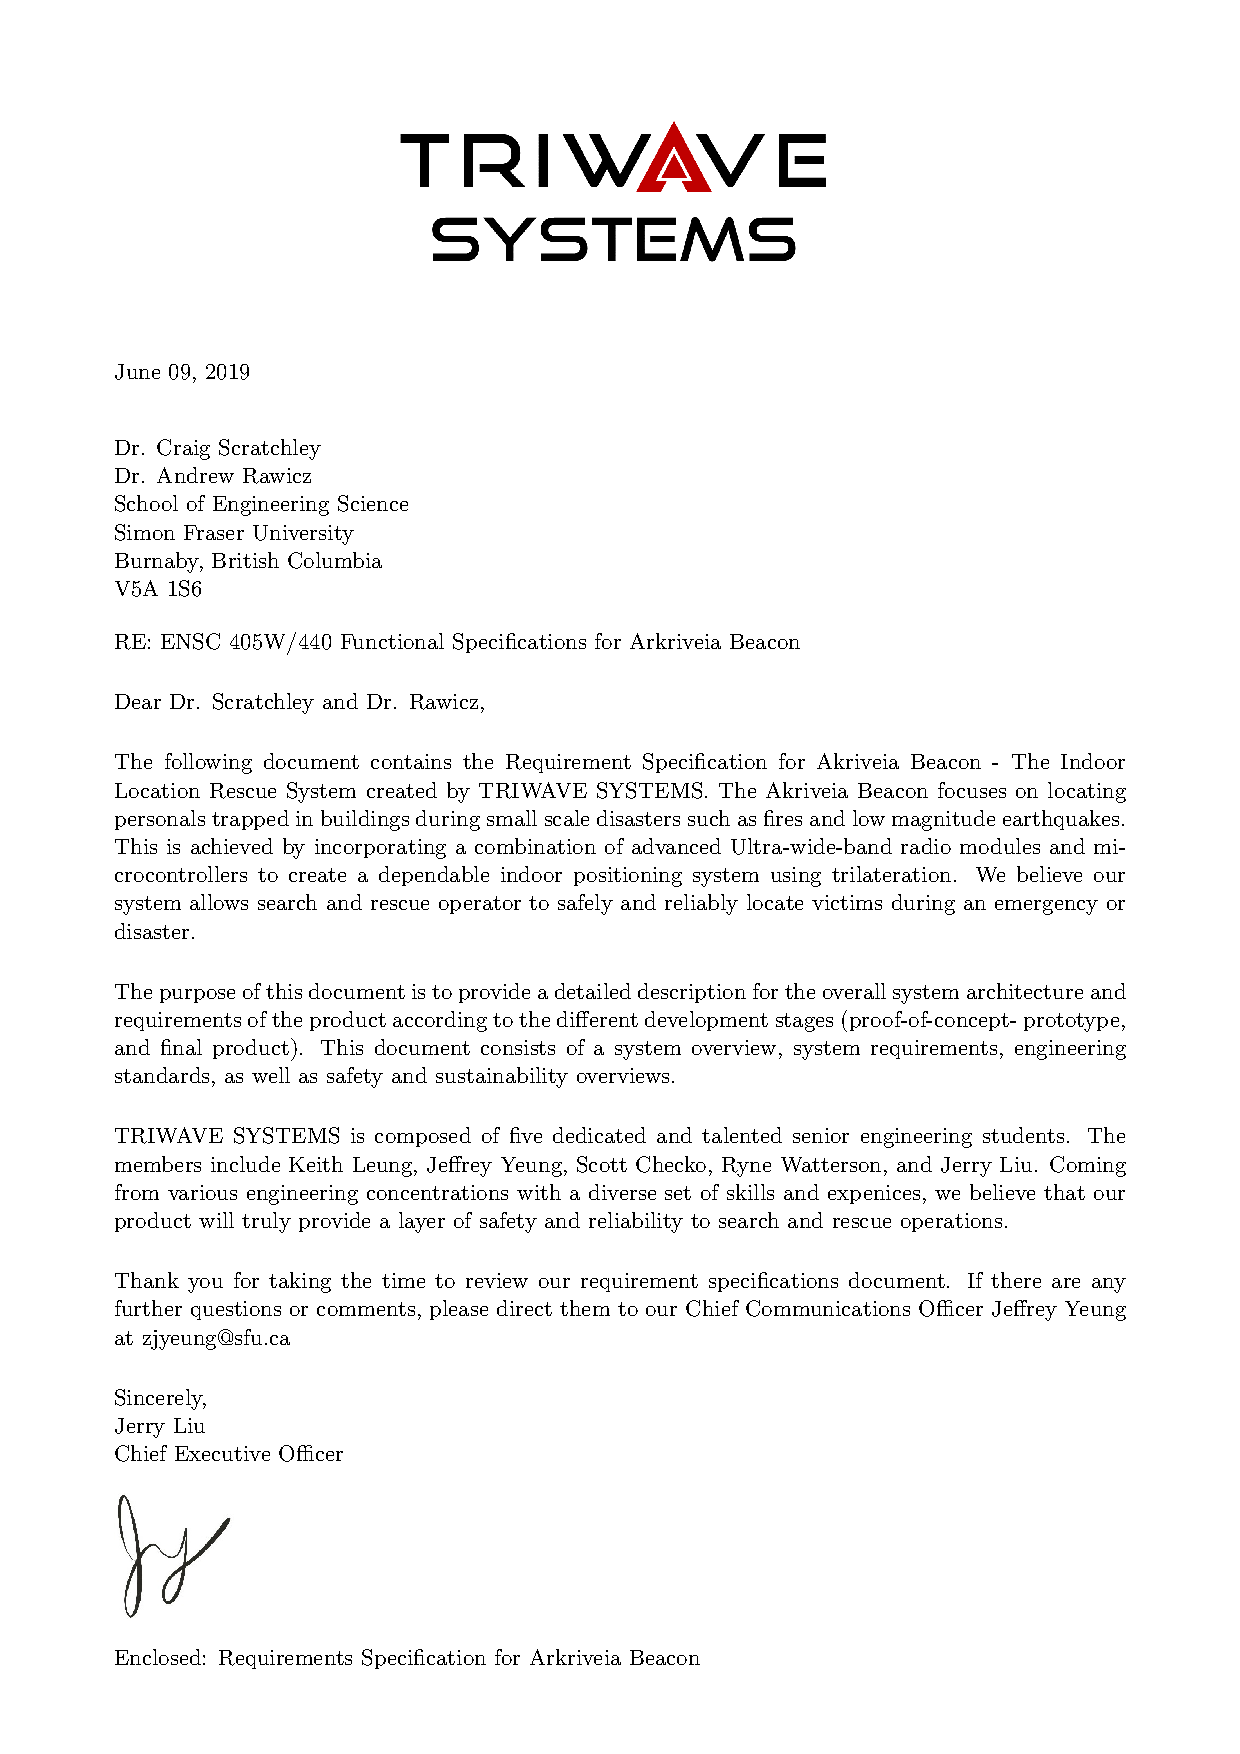
\includepdf[pages={1}]{./images/__Letter_of_transmittal.pdf}
%\setboolean{@twoside}{false}
%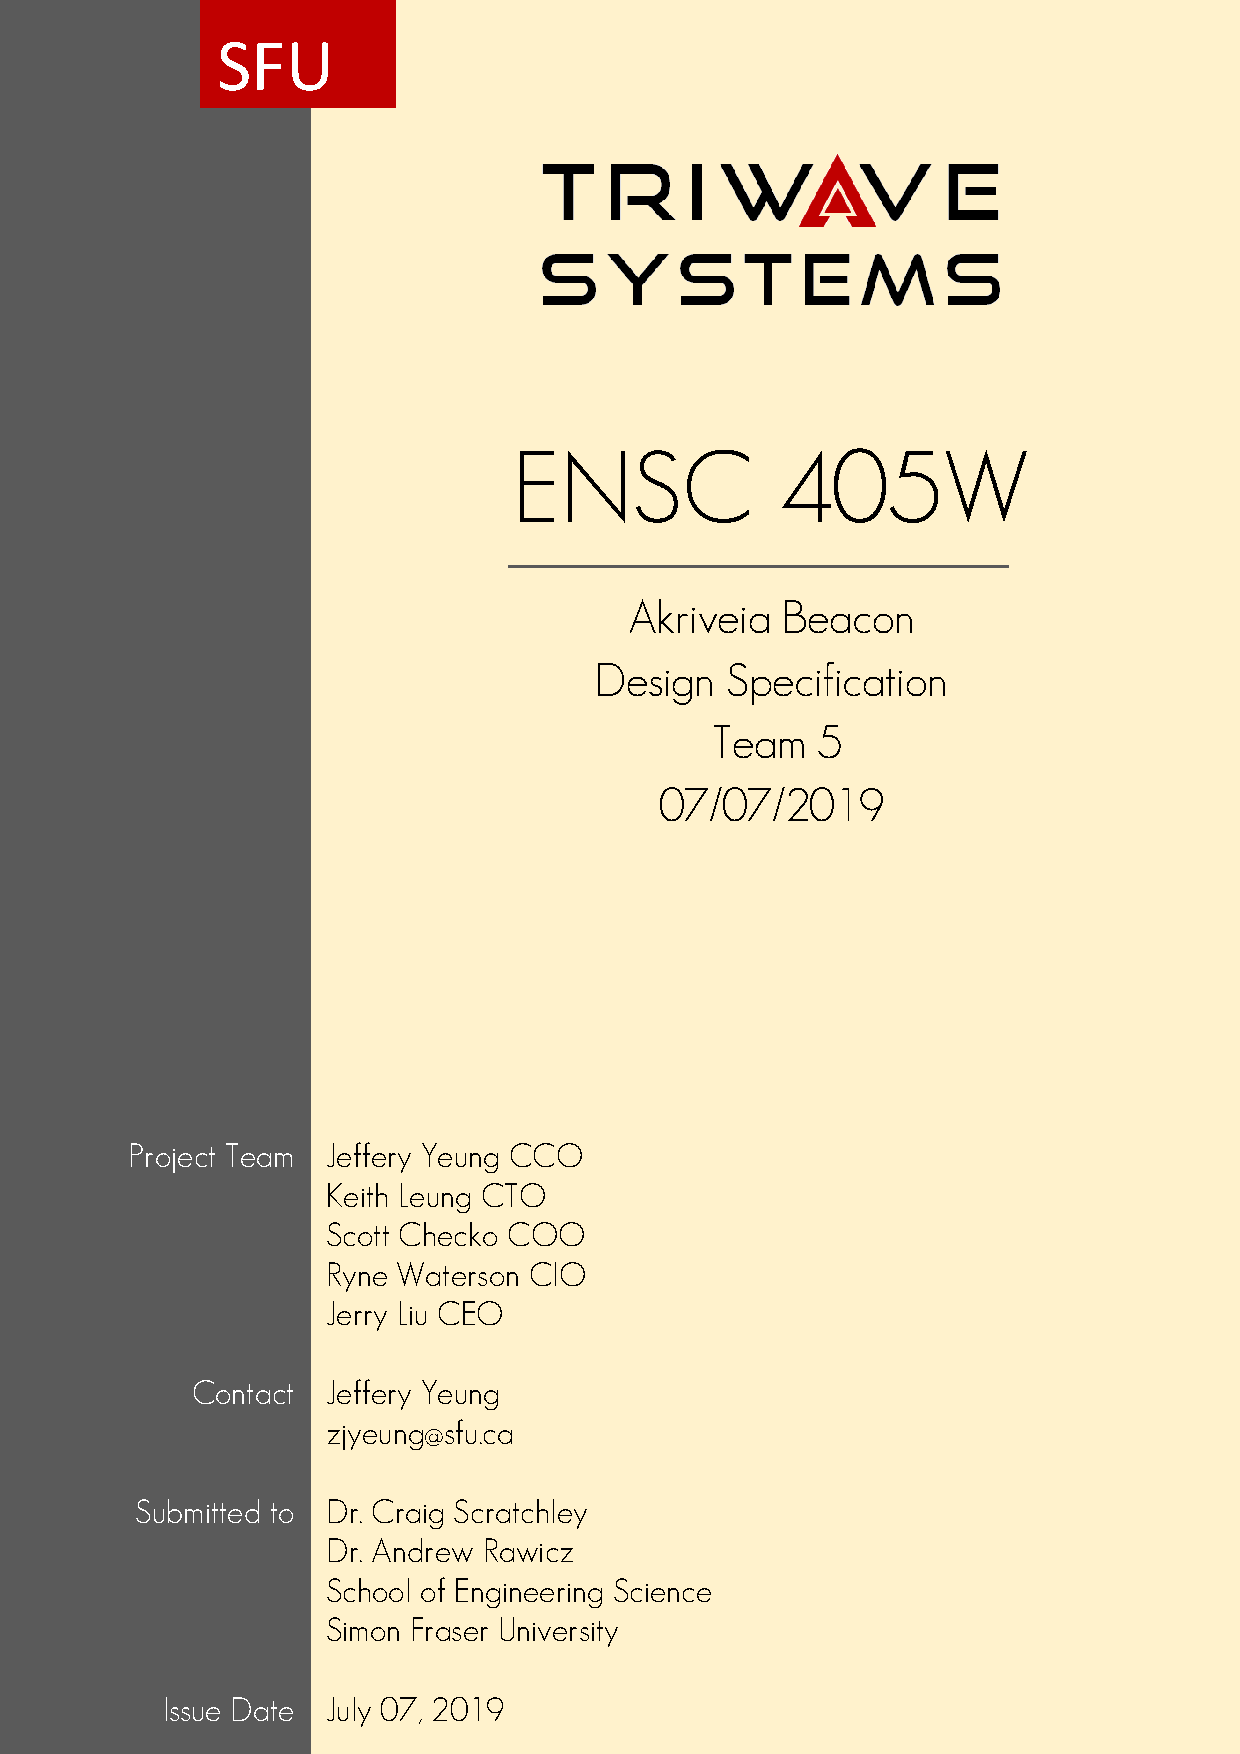
\includepdf[pages={1}]{./images/title_page.pdf}
\


\section*{Executive Summary}	%For left alignment of title
\bigskip
A major concern during disaster search and rescue operations involving large and complex commercial buildings is the process of locating potentially trapped victims. In current conventions, there are no reliable methods of accurately locating trapped victims for first responders, as commercial building structures are large and complex by design. The Akriveia Beacon by TRIWAVE SYSTEMS focuses on creating an safe and dependable solution for indoor location tracking with the objective of locating multiple trapped victims in complex urban environments with pin point accuracy. Such system will allow search and rescue operations to be carried out during small scale disasters such as fires and low magnitude earthquakes safely and efficiently, minimizing potential damages and casualties.

\bigskip
Utilizing various hardware, electrical and software components, the engineers at TRIWAVE SYSTEMS is aiming to create a solution that can accurately and reliably to locate and identify trapped victims within complex structures in near real time. By pinpointing the exact coordinates of any trapped victims associated with an ID tag, the search and rescue time for first responders can be minimized, which is critical in any disaster rescue operations. This is achieved by incorporating a combination of advanced Decawave Ultra-wideband radio frequency (\Gls{RF}) modules, Espressif ESP32 microcontroller units (\Gls{MCU}), data processing units (\Gls{DPU}), and reliable trilateration techniques to create a dependable real time indoor location positioning system.

\bigskip
This project proposal document provides a brief overview of the system architecture; perspective on current markets and potential competitions; discuss project planning; available budget, funding, and cost consideration; as well as an overview of the development team at TRIWAVE SYSTEMS. The proposal will cover the three phases of product development: Proof-of-concept (\Gls{PoC}) phase, Prototype phase, and Final Product phase.

\bigskip
TRIWAVE SYSTEMS is dedicated to creating a reliable and robust indoor location system designed to improve disaster search and rescue operations with human safety as the pivotal focus.

\pagebreak
\clearpage
\printglossaries
\pagebreak
\begin{spacing}{0.90}
\tableofcontents
\end{spacing}
\pagebreak
\listoffigures
\pagebreak
\listoftables
\pagebreak


\setcounter{section}{0}
\section{Introduction}
\bigskip

\subsection{Background}
Over the last couple of decades urban centers around the world have faced substantial population growth. As a result, the number of large and complex structures in dense urban areas around the world is rapidly increasing. In Canada alone there are approximating 500,000 commercial buildings \cite{R1}. A large population combined with massively complex buildings in relatively dense areas leads to higher risk for damage and casualties in the event of a disaster. Due to increased urbanization and complexity of urban structures, search and rescue operations in indoor urban environments face various complications and uncertainties. According to Statistics Canada, an average of 135 fire related deaths occur with commercial structures each year from 2010 to 2014 \cite{R2}.

\bigskip
In current practices, first responders know little about the situation until arriving on scene. Once responders are on scene, emergency management have to quickly evaluate the situation and take appropriate actions \cite{R3}.  Assessments of the structure are conducted with readily available blueprints of buildings along with limited information of last known location of possible trapped victims, usually derived from witness reports. Situational data are created dynamically during this process and the actual rescue process heavily depends on the situational awareness of the first line of emergency response operators \cite{R4}.

\bigskip
An important issue that must be considered is how emergency first responders should be dispatched inside the building in the event of a disaster in order to minimize search and rescue time. In order to pinpoint locations of trapped victims quickly and accurately it is critical to have precise data. Proper emergency planning and organization takes a substantial amount of time, and having additional accurate information on the locations of trapped, incapacitated or immobile personnel would improve first responders situational awareness which would then improve their own safety and possibly greatly increases the victims chances of rescue and survival.

\bigskip
As such, the need for a distinct indoor positioning rescue system is crucial in getting fast and reliable information that allows first responders to be dispatched within the builds in the most optimal and efficient manner. The Akriveia Beacon by TRIWAVE SYSTEMS focuses on improving the locating and rescue process of personnel trapped in buildings during or after small scale disasters such as fires and low magnitude earthquakes. This is done through a system of Ultra Wide-Band (\Gls{UWB}) Beacons and \Gls{ID} tags for accurate, near real-time location of trapped personnel.

\bigskip
Ultra-Wideband radio modules are small radio transceivers using ultra-wide band radio spectrum to communicate with one another. Each ID tag uses a UWB transceiver module to communicate with the beacon system with similar UWB transceivers. Given the time between sending and receiving transmission data, the distance can be estimated via \Gls{RSSI} or time of flight. The Beacons will then forward these distance estimations to a data processing unit using a closed Wi-fi network where it will use trilateration to calculate the near real time location of each individual ID tag. The system design allows for multiple ID tags as well as more than three anchor beacons to provide more accuracy through redundancy, making it modular and extendible.

\break
\subsection{Scope}
\medskip
The Akriveia Beacon product is developed through three different phases of development as shown in Figure \ref{dev}. The three different phases including: the proof-of-concept phase, prototype phase, and final product phase. A high-level design of the system hardware and software is presented in this document to demonstrate the overall system architecture, functionality and implementation of the Akriveia beacon product. The design section of this document is divided into four main sections, overall system design, hardware design, electrical design, and software design. These design specification will indicate the components, implementations, requirements, and constraints that must be met and satisfied within the project time frame. 

\medskip
\begin{figure}[H]
\centering
    
\includegraphics[scale=0.5]{./images/dev-path.png}
    \caption{Development Cycle}
    \label{dev}
\end{figure}


\subsection{Intended Audience}
\medskip
This document is presented by engineers at TRIWAVE SYSTEMS as a guide for the design and system overview of the Akriveia Beacon product. The intended audience of this document includes but not limited to, potential clients and/or partners, the supervising professors Dr. Craig Scratchley and Dr. Andrew Rawicz, associated teaching assistants and fellow TRIWAVE SYSTEMS members. The hardware and software engineers of the project can reference this document during the various stages of development and testing stages of the project for clarification. Near the completion of the prototype development phase the product will be tested against the cases specified in the test plan. Engineers responsible for performing quality assurance can refer to the Appendix of this document to ensure all safety concerns have been addressed and that the product fulfils all requirements and meets all expectations for proper usage. 

\break
\subsection{Design  Classification}
For consistency purposes, the following design classification code convention is used to describe and organize design requirements listed throughout this document. 
\medskip
\begin{center}
	\textbf{[ DES.SE.\# - X ]} 
\end{center}

\bgroup
\def\arraystretch{1.5}
\begin{table}[H]
\centering
\begin{tabular}{ | m{1cm} | m{13cm}| } 
\hline
\rowcolor{lightgray} \textbf{Code} & \textbf{Definition} \\ 
\hline
 \textbf{DES} & Design abbreviation. \\ 
\hline
 \textbf{SE} & Design Domain Abbreviation Code correspond with each Design requirements. (see Table 2)\\   
\hline
 \textbf{\#} & Design number ID \\ 
\hline
 \textbf{X} & Development Stage Encoding (see Table 3)\\ 
\hline
\end{tabular}
\caption{Design Requirement Encoding}
\end{table}

\bgroup
\def\arraystretch{1.5}
\begin{table}[H]
\centering
\begin{tabular}{ | m{7cm} | m{7cm}| } 
\hline
\rowcolor{lightgray} \textbf{Requirement Domain} & \textbf{Abbreviation Code} \\ 
\hline
 System & SY\\ 
\hline
 Hardware & HW\\ 
\hline
 Electrical & EC\\  
\hline
 Software & SW\\ 
\hline
\end{tabular}
\caption{Design  Domain Abbreviation Code}
\end{table}

\bgroup
\def\arraystretch{1.5}
\begin{table}[H]
\centering
\begin{tabular}{ | m{7cm} | m{7cm}| }
\hline
\rowcolor{lightgray} \textbf{Development Stage} & \textbf{Encoding} \\
\hline
Proof of Concept & C\\
\hline
Prototype & P\\
\hline
Final Product & F\\
\hline
\end{tabular}
\caption{Development Stage Encoding}
\end{table}	













\pagebreak


\setcounter{section}{1}
\section{System Overview}
\bigskip

The Akriveia Beacon indoor locating rescue system combines hardware, electrical, and software systems to detect and locate multiple occupants within a building during an emergency disaster situation. Each individual component of the system is developed separately in the PoC (Proof of Concept) phase; then partially integrated in the Prototype phase and fully integrated in the Final Product phase. 

\bigskip
A high-level system overview presents three Locator Beacons, an ID tag, a data processing unit, and a graphical user interface (Figure \ref{sys_arch}). Using ultra-wideband (3.5-6.5 GHz) wireless communication the Locator Beacons transmit signals to the ID tag to acquire a response. When the response returns back to the Beacon a time of flight measurement is acquired. The Time-of-Flight principle (ToF) is a method for measuring the distance between a sensor and an object, based on the time difference between the emission of a signal and its return to the sensor, after being reflected by an object. \cite{R2-0}. The ToF data will be forwarded to the portable data processing unit via a closed Wi-Fi network with UDP.  Then the processing unit will calculate the distance and coordinates of the ID tags using trilateration algorithm. Afterwards, the coordinates results are displayed on a GUI for operators.

\medskip
\begin{figure}[H]
\centering
    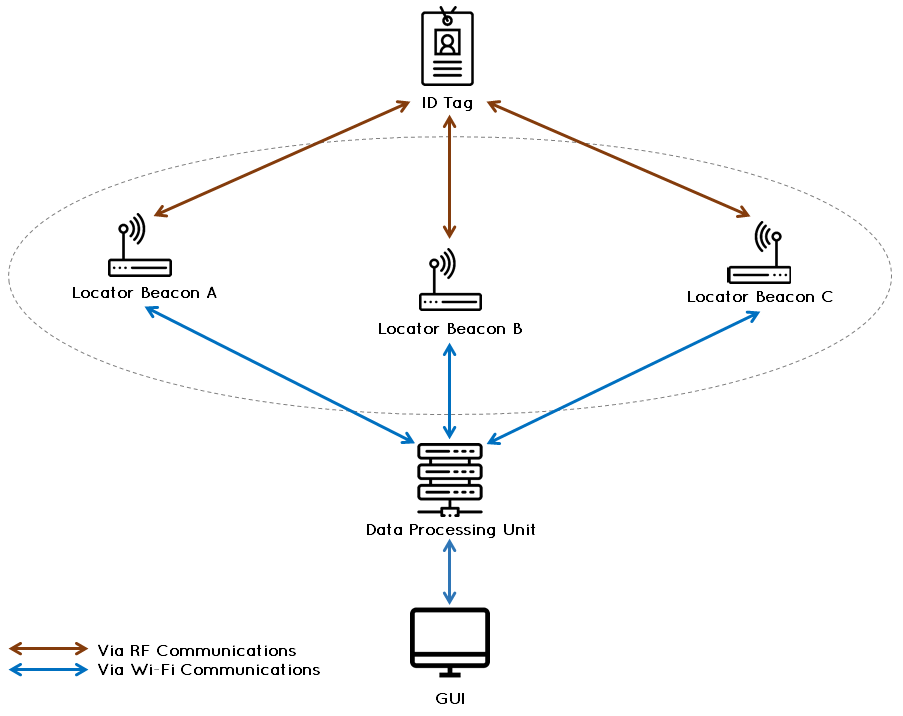
\includegraphics[scale=0.65]{./images/00_sys_arch.png}
    \caption{High Level System Layout}
    \label{sys_arch}
\end{figure}



\pagebreak
\subsection{Proof of Concept}
\medskip
The Proof of concept phase demonstrates the feasibility and functionality of an indoor location determination system. The PoC system will evaluate how effect a trilateration method is to determine the distance and location of a mobile  ID tag in two dimensional space as well as to establish an initial development system. Similar to the system block diagram shown in figure \ref{poc}.

\bigskip
ESP32 micro-controllers are used as the main hardware components of the Beacon and ID Tags. The ESP32 is an off the shelf, low-cost, low-power system on a chip micro-controllers with integrated Wi-Fi and dual-mode Bluetooth. Received Signal Strength Indicator (RSSI) from Bluetooth Low Energy (BLE) modules are used to estimate distance between each beacon and ID tag. Each beacon determines the MAC address and a RSSI measurement from the advertising ID Tag. The data is forwarded to the data processing unit - Raspberry Pi, via USB serial communication. The RSSI is then used to estimate distance between each ID Tag and the associating Beacon and the results are output to a simple UI. 

\medskip
\begin{figure}[H]
\centering
    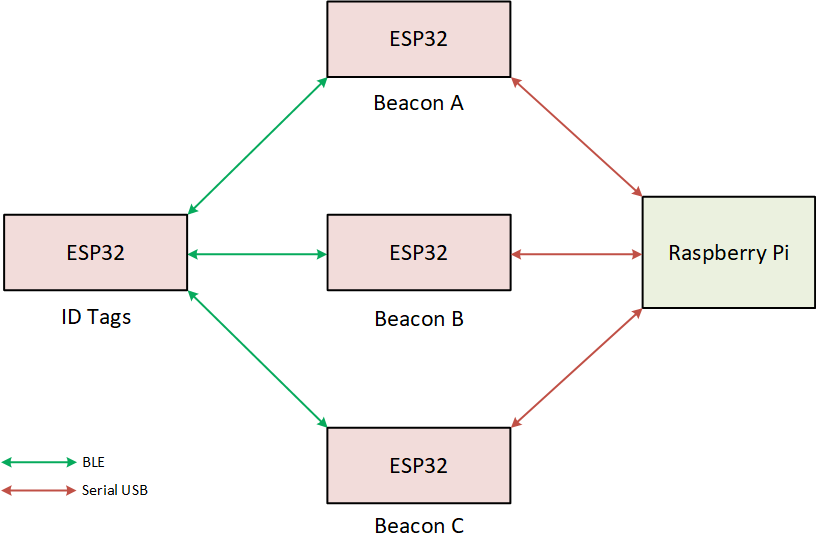
\includegraphics[width=\linewidth]{./images/01_poc.png}
    \caption{PoC System Block Diagram}
    \label{poc}
\end{figure}



\pagebreak
\subsection{Prototype}
\medskip
In the Prototype development phase the transceivers will be incorporated with Decawave DWM1000 UWB modules. The DWM1000 UWB uses radio frequencies in the range of 3.5 to 6.5 GHz; this would significantly reduce issues of signal interference or multipath propagation which would occur by using RSSI with BLE. The DWM1000 will be incorporated as the transceiver with the ESP32 as the main MCU as shown in figure \ref{prototype} below. RF data communication functions will be established between four UWB modules with one as the ID Tag and three as the Locator Beacons to demonstrate distance estimation with DWM1000 UWB modules. This will be achieved by using signal fingerprinting to determine transmitter properties such as ToF and unique Tag identifier. Furthermore, trilateration algorithms will be implemented on data processing unit to determine near real time location and coordinates of ID Tags. Initial Implementation of software stack on data processing unit and development of GUI will occur during this phase as well.

\medskip
\begin{figure}[H]
\centering
    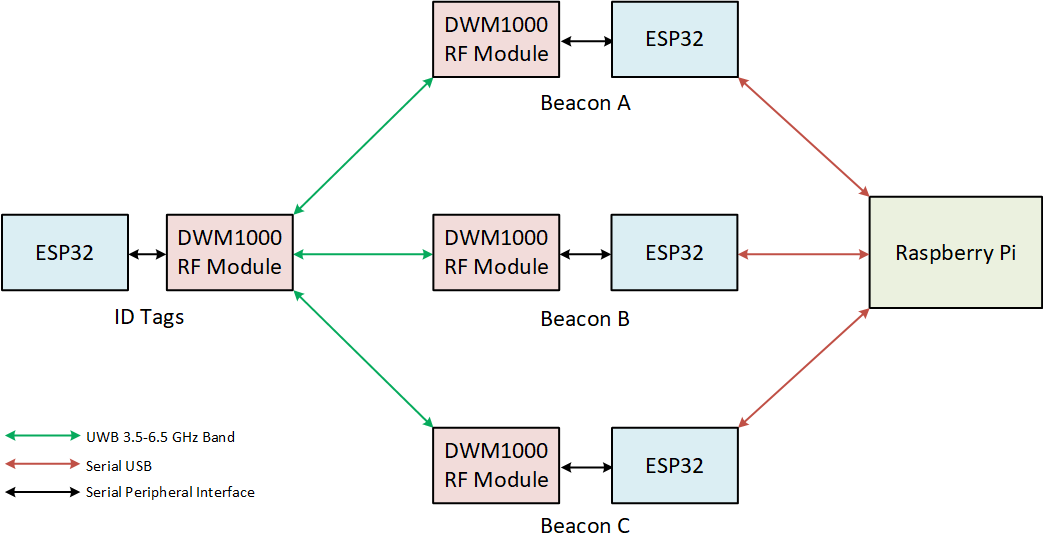
\includegraphics[width=\linewidth]{./images/02_prototype.png}
    \caption{Prototype System Block Diagram}
    \label{prototype}
\end{figure}


\pagebreak
\subsection{Final Product}
\medskip
The final product will demonstrate the fully functional indoor rescue system that detects the location of the ID tags and displays it accordingly on a GUI. Here the addition of ESP32’s Wi-Fi modules can be seen (Figure \ref{final}), as the Beacon will communicate via Wi-Fi communication with the data processing unit. The Wi-Fi network will be a closed network meaning that the network is only share between beacons and the data processing unit to ensure security, reliability and stability. Furthermore, implementation of RF harvesting circuit for ID Tag device charging during deep sleep mode will occur during this stage. All the components of the systems will be fully integrated as a close-to-production product. Component circuits and PCB footprint will be minimized and proper casing will be made to house all electronics. The data processing unit will provide the user with a full GUI to interact with the system along with the fully implemented features such as importable blueprints and multi-floor tracking.

\medskip
\begin{figure}[H]
\centering
    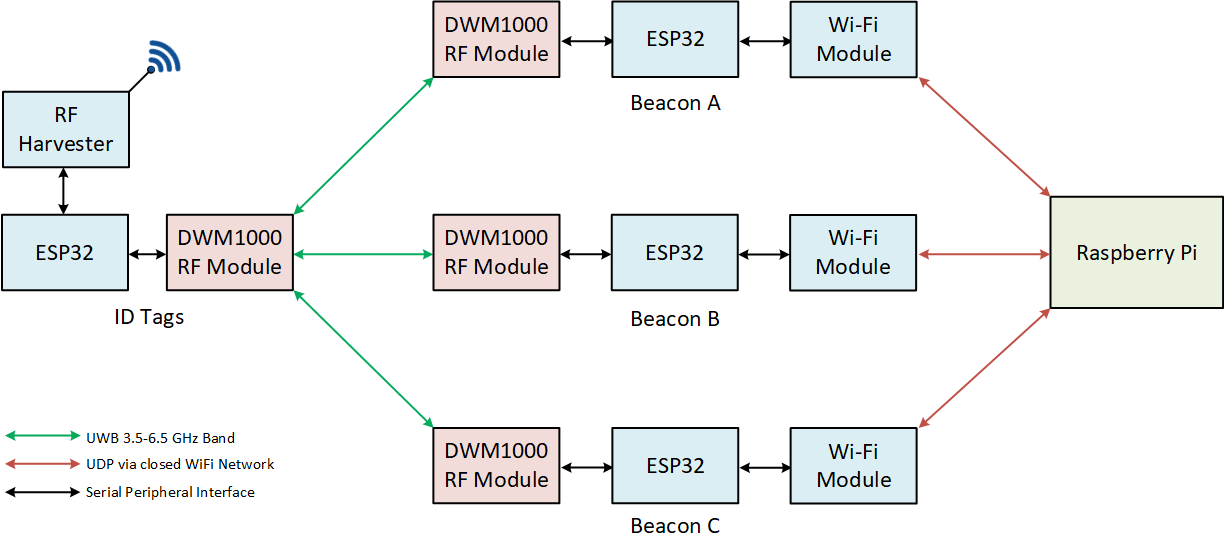
\includegraphics[width=\linewidth]{./images/03_final.png}
    \caption{Final System Block Diagram}
    \label{final}
\end{figure}




\pagebreak
\subsection{Ultra-Wideband Radio Technology}
\medskip



\pagebreak
\subsection{Trilateration Methods}



\pagebreak


\setcounter{section}{2}
\section{Current Market \& Competitions}

%-----Markets-----$
\subsection{Markets}
Currently there are two major markets available for Global Indoor Location (\Gls{GIL}) and Search and Rescue (\Gls{SAR}) equipment. 
The Global Indoor Location market is worth \$ 3.43 billion in 2015 and is projected to reach \$ 29.4 billion in 2022 \cite{R3-1}. This advent 
comes from the increasing amount of smartphone users and ineffective Global Position Systems (\Gls{GPS}) for indoor use. On the other hand, SAR market 
worth is projected to rise from \$ 113.62 billion in 2017 to \$ 125.66 billion by 2022 \cite{R3-2}. Mainly the increased focus on citizen 
safety and rising terroism/insurgency threats supports the upward trend. Suprisingly, UWB is only utilized for GIL market for commercial use in 
warehousing, breweries, factories and other various applications. However, none uses UWB for GIL in emergency situations as SAR equipment. 
Therefore, Triwave Systems uniquely positions itself between two multibillion dollar markets, GIL and SAR, and allowing freedom to compete in both. 

\bigskip

There are multiple Global Indoor Location (GIL) systems available on the market. Each GIL system relies on their own specific technology and has 
their own benefits and cons. Based on the journal \textit{Localization and Positioning Systems for Emergency Respondiers: A Survey}\cite{R3-3}, 
there are five categories or attributes on which each GIL are evaluated: Accuracy, Information Accessibility, System Adaptability, System 
Architecture, System Autonomy and Cost. Of the numerous technologies stated in the journal, only UWB provides the sufficient accuracy and 
reliability needed for indoor tracking for individuals during emergencies. In fact, UWB if optimized properly can provide the necessary <1m 
accuracy compared to other technologies. UWB operates on the frequency range from 3 – 6 Ghz band which enables higher accuracy, less interference 
and multipath propagation effect. Bluetooth and Wifi utilize 2.4Ghz which severely reduces its accuracy due to multi-path propagation effect 
and interference. Although 2.4Ghz frequency GIL sysytems are inexpensive and readily available, the inconsistent nature of RSSI causes Wifi and 
Bluetooth GIL systems to be inaccurate \cite{R3-4}. UWB although more costly, can provide the necessary location tracking that our emergency 
tracking system requires. Thus, UWB technology is the most appropriate for our specific scenarios and use cases.

%----Competition-----%
\subsection{Competition}
There are a number of competitors in the market that uses the same UWB technology for indoor localization as Triwave Systems. 
However, the application of their products is mainly associated with tracking equipments and items in warehouse or production facilities, 
which differs from the scope of search and rescue and does not compete directly with our product. The various companies, infsoft or Pozyx, use 
UWB for tracking individuals in warehousing. Tracking individuals or items in non-emergency situations do not necessitate the need for high 
precision localization. As well, use cases where power is out are not considered in the product specifications as vital. UWB applications in non 
life-threatening situations do not demand such strict regulation or procedures compared to SAR equipment. Triwave Systems' Akriveia also has 
backup battery power for the beacons in case of emergencies. Since the ID tags are mainly in deep sleep waiting for user input and the beacons 
emergency broadcast, these ID tags can last several years in deep sleep considering optimal conditions \cite{R3-5}. Another defining feature for 
Akriveia systems is the integrability of the ID tag with the access card. There will be no need for employees to carry two separate cards but 
rather one card with both functions. 

%---update the reference numbers --------------------%
\subsubsection{infsoft}
infsoft is a competitor that provides indoor tracking solution mainly to industrial environments using UWB sensors. 
Similar to Triwave Systems, their tracking system consists of two components: locator tags and locator nodes, for which the locator tags 
can be attached to people or objects and the locator nodes are installed at fixed locations in an infrastructure. Some suggested uses cases 
for their UWB locating systems are forklift localization, route analysis, asset tracking and tugger train management, which are mainly in 
warehouse or production facilties \cite{R3-6}. In applications where locator tags are attached to immobile objects such as asset tracking, 
such a system would be beneficial as it may prevent incorrect inventories. However, in applications where the locator tags are attached to 
people such as search and rescue, privacy becomes an issue as their navigation within the coverage area of the locator nodes are exposed in 
real time. Triwave Systems ensures that user privacy is preserved in all non emergency situations by preventing ID tags to broadcast signals 
which forbids data reception from our beacons. This solution also decreases power consumption of ID tags significantly, hence lengthening 
their battery life as well. 

\subsubsection{Pozyx}
Pozyx is another company that provides tracking solutions using UWB technology for production and other industries. With the same system 
components as of infsoft, the company categorizes its products in two families: Creator and Enterprise. The Creator kit pricing at 
\EUR{1050} consists of 4 tags and 5 anchors is aimed for hobbyist prototyping purposes, whereas the Enterprise kit pricing at \EUR{3900} 
consists of 3 tags and 6 anchors is used in large industrial environments \cite{R3-7}. In terms of accessibility, both product families may 
not be ideal for their dedicated comsumers due to their high price points. Despite difference in use case, Triwave System integrates 
components that are less costly to build ID tags and beacons in order to maintain a widely accessible yet cost effective system. 

\subsubsection{Articles/Journals}
Instead of tags and anchors, the wireless sensor invented by the King Abdullah University of Science and Technology is a handheld portable 
device engineered to detect human body movements such as respiratory chest movements with UWB technology. It is low cost solution with high 
level of accuracy and the ability to penetrate obstacles due to benefits of UWB technology, which is seemingly ideal for search and rescue 
\cite{R3-8}. However, problems arise due to the handheld nature of the device in search and rescue. Firstly, the chance of locating victims
is highly dependent on the coverage area and direction of the search conducted by the device user. This human dependency may pose limitations 
to its effectiveness on search and rescue since it is difficult to have full coverage on a disaster site. Lastly, having an extra device to 
carry can also be an extra burden to first responders who carries gears and equipment during a search operation. Triwave Systems solves these 
problems by having UWB sensors attached to potential victims instead of first responders. Search coverage is also handled by the distribution 
of our beacons and our data processing unit allows first responders to locate victims more effectively without carrying a device into dangerous 
environments.

\bigskip
One article \textit{Indoor localization for evacuation management in emergency scenarios} discusses about using a WiFi system that computes 
indoor localization to the person’s phones \cite{R3-9}. The sensors that detect smoke would send an alarm to the web server which would in turn 
send alerts to Rescuer apps and Worker apps. The phone app would guide the person to exits or provide emergency assistance. However, the authors 
exaggerate the effectiveness and accuracy of RSSI. Thus, the article only provides the concept of an Emergency Indoor Localization system without 
physically implementing it. 

\pagebreak


\setcounter{section}{3}
\section{Budget \& Funding}
\bigskip


\pagebreak


\setcounter{section}{4}
\section{Project Planning}
\bigskip

The development of the Akriveia Beacon system will go through three different phases of development: the Proof of Concept phase, the Prototype phase, and the Final Product phase. The development of these three phases will span over a time period of  eight months (two semesters), starting from May 2019 and ending in December 2019 as shown in the project milestone chart in figure \ref{mile}. 

\bigskip
The Proof of Concept phase will be delivered at the end of the first four months (first semester) in August 2019. The Prototype  phase will be complete in October 2019 (in the middle of the second semester). Lastyly, the Final Product phase will be delivered at the end of the eight months (two semesters) in December 2019. 

\bigskip
The 405W project development timeline can be viewed in the Gantt chart presented in figure \ref{gantt}. This Gantt chart details the tasks and milestones associated with the proof-of-concept development phase of the Akriveia Beacon system. This Gantt chart does not include tasks and milestones in 440 as the timeline for 440 is unclear at the writing of this document. Furthermore, the two tasks, Prototype UWB Testing and Prototype UWB System Integration listed under number 21 and 22 respectively, will continue into 440 as UWB development will continue past the PoC development phase.

\medskip
\begin{figure}[H]
\centering
    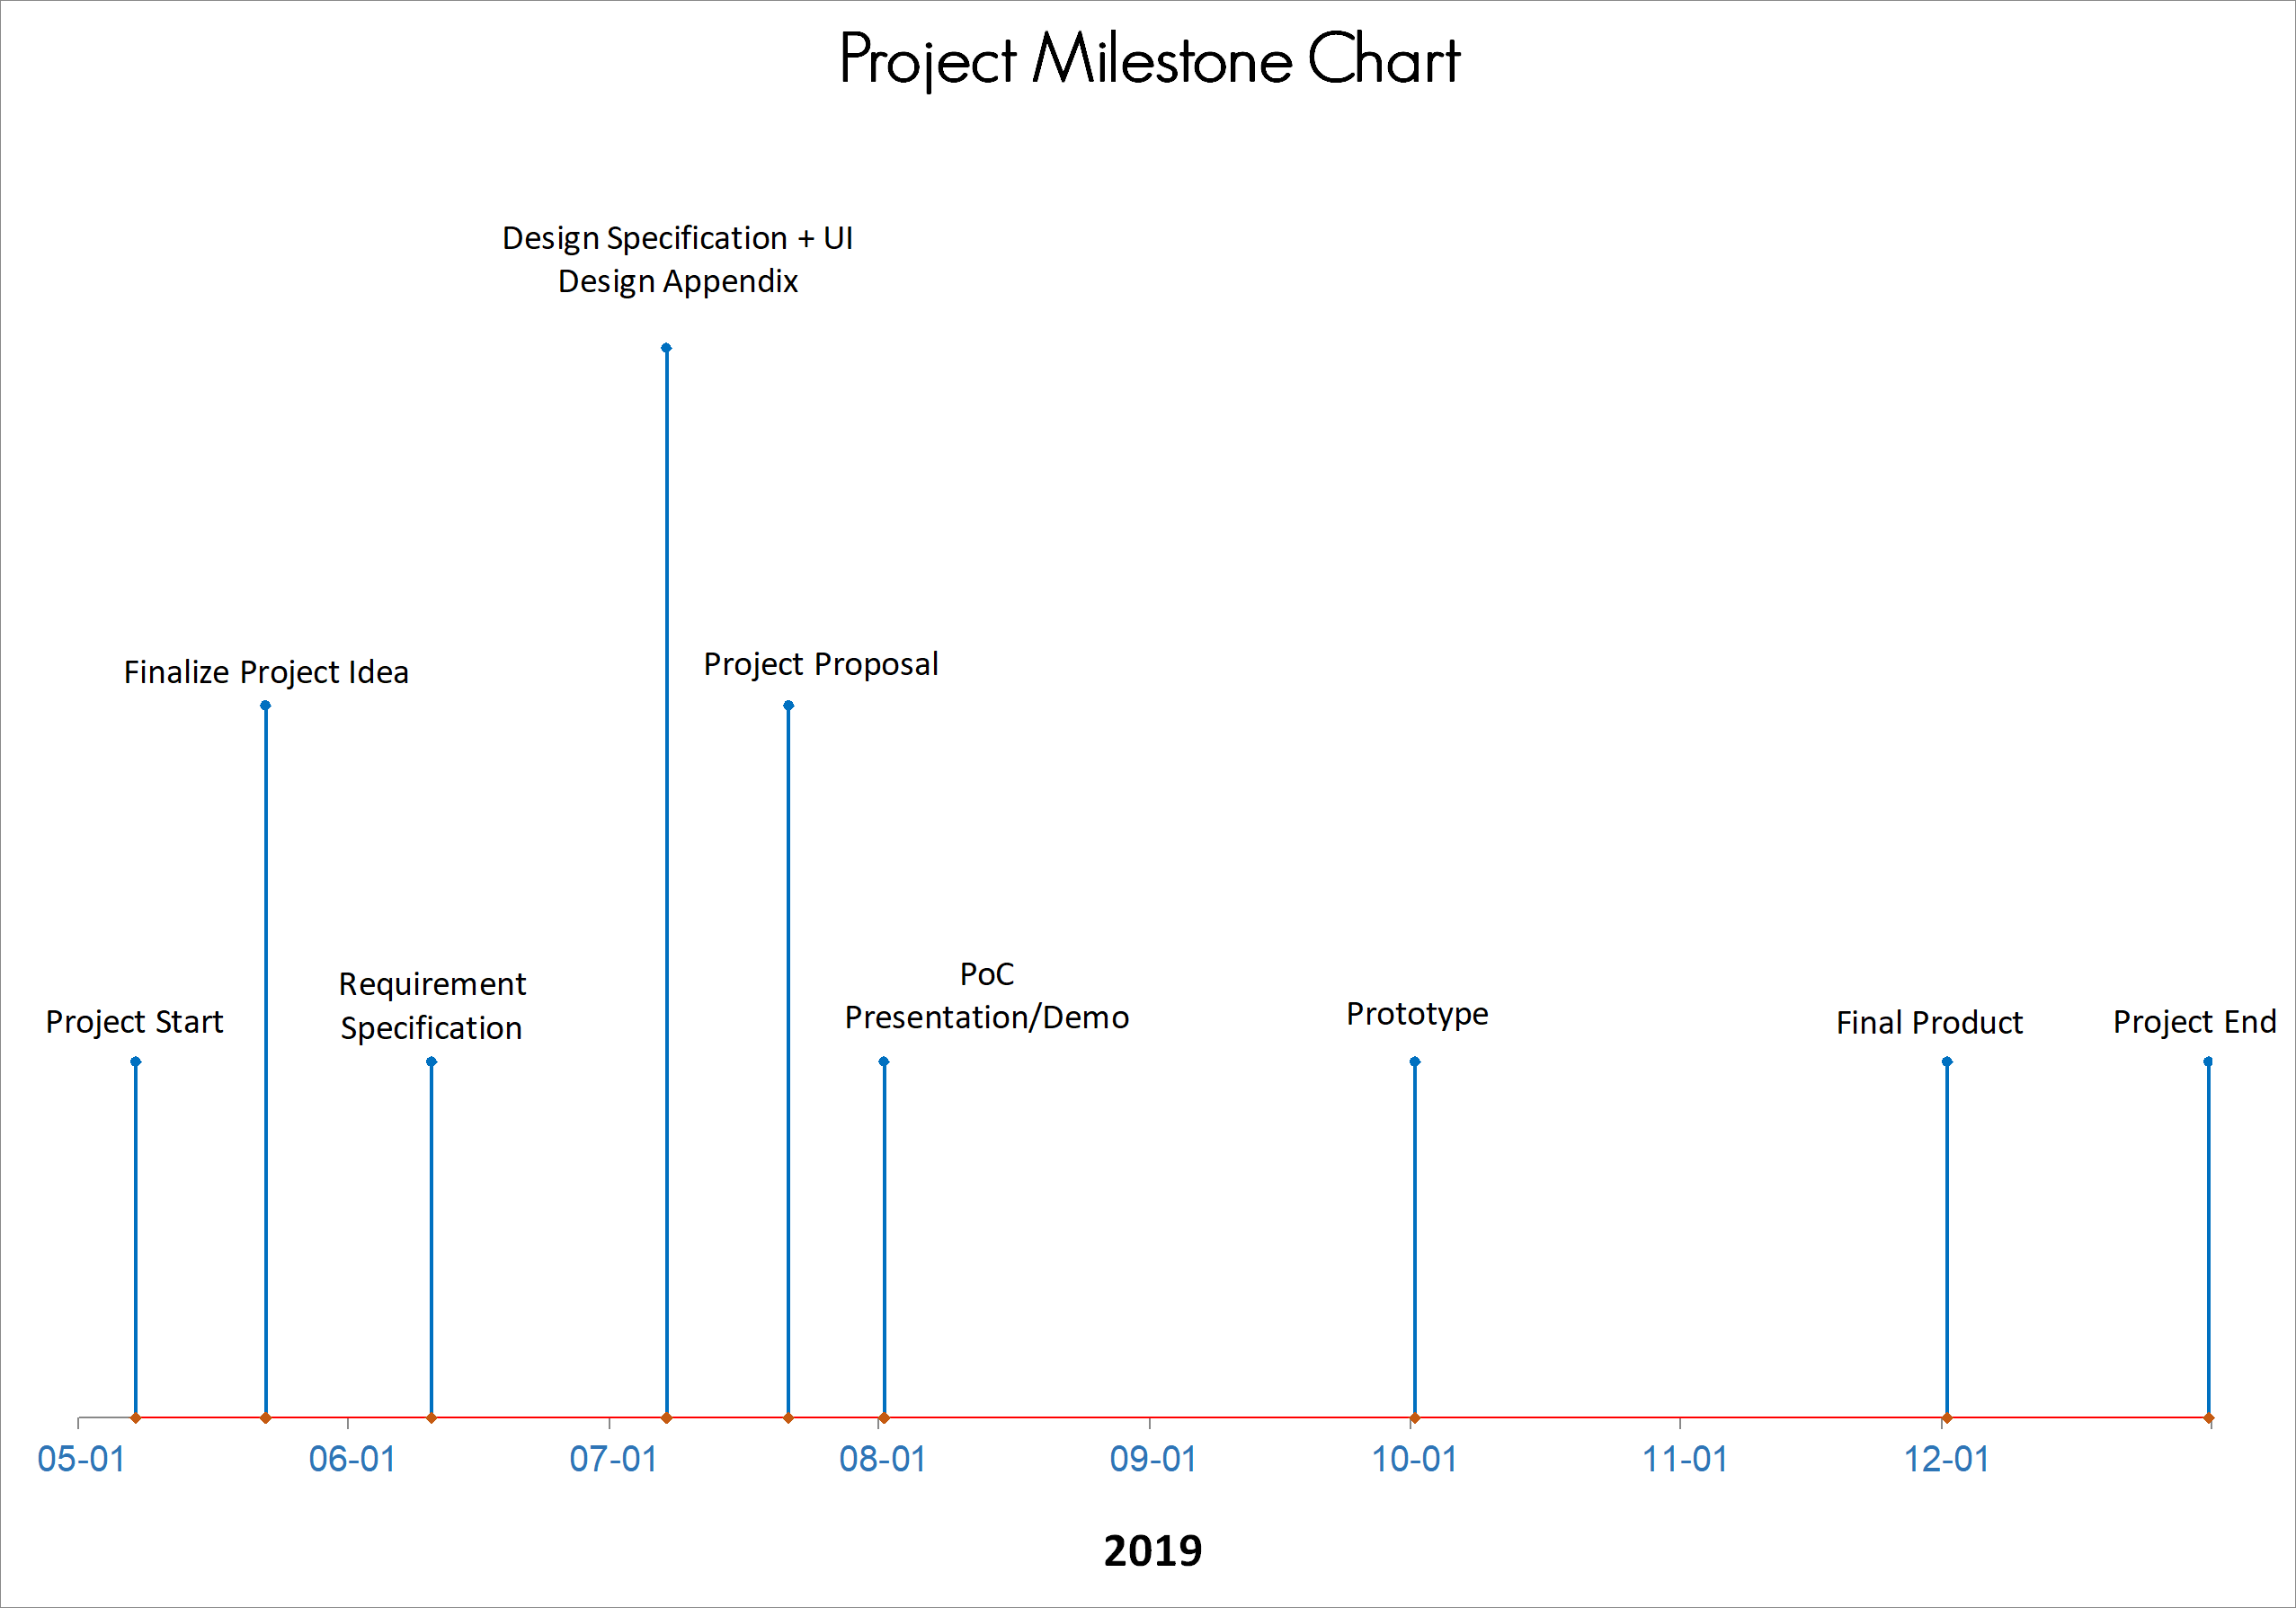
\includegraphics[width=\linewidth]{./images/mile.png}
    \caption{Project Milestone Chart}
    \label{mile}
\end{figure}

\pagebreak
\thispagestyle{empty}
\newgeometry{bottom=2cm,left=2cm,right=2cm,top=2cm}
\begin{landscape}

\begin{figure}
\centering
    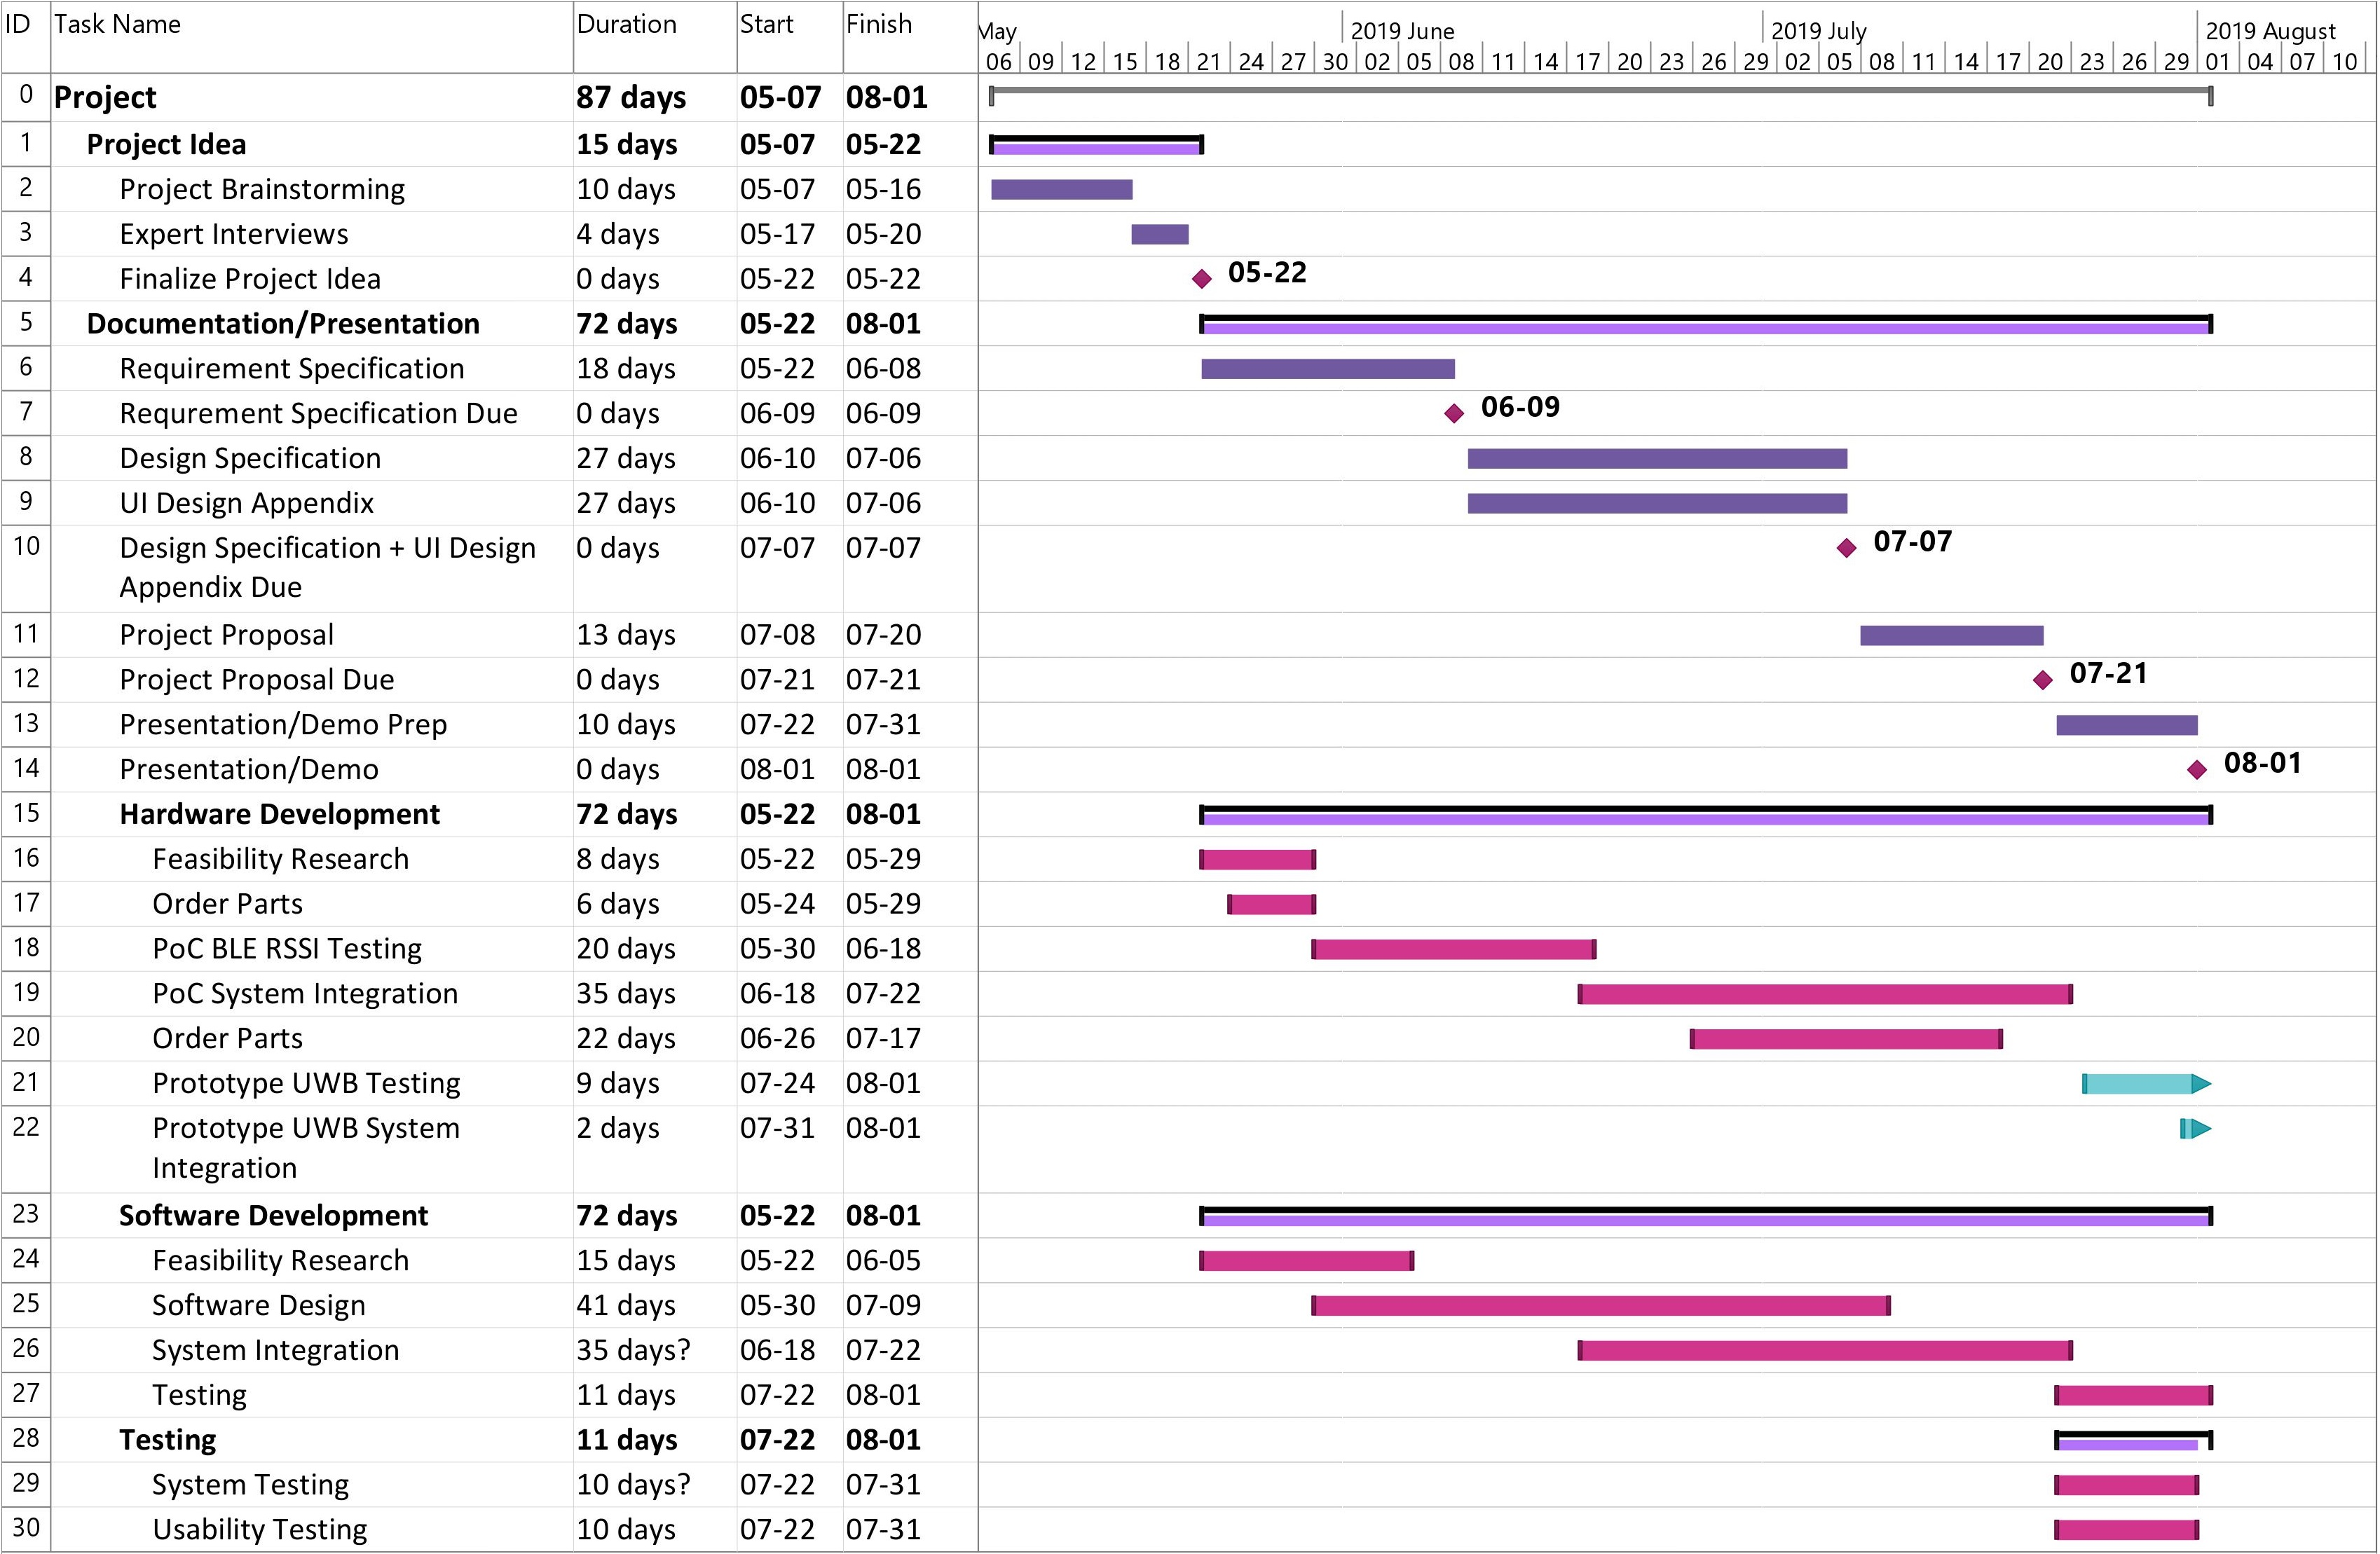
\includegraphics[width=\linewidth]{./images/gantt.jpg}
    \caption{Project Gantt Chart}
    \label{gantt}
\end{figure}
\restoregeometry
\end{landscape}





\pagebreak


\setcounter{section}{5}
\
\section{Company Details}

\bigskip
\textbf{Name} Jeffery Yeung \\
\medskip
\textbf{Title}: Chief Communications Officer (CCO)\\
\medskip
\textbf{Background}:
Jeffery is a sixth year engineering science student at SFU pursuing a degree in Systems Engineering. His previous experience includes 
working at Mix Technology Inc. in Hong Kong and Integral Group in the Vancouver office. He has gained valuable experience in PLC software
design and gained valuable insight into Hong Kong's diverse and booming construction industry. His time at Integral Group further cemented
his understanding of building verification and the importance of proper building commissioning. He hopes to apply his acquired skills and experience
in the construction industry towards machine learning for building HVAC. His goal is to reduce building HVAC energy consumption and 
advance sustainability or green practices in building design.

\bigskip
\bigskip
\textbf{Name}:  Keith Leung\\
\medskip
\textbf{Title}: Chief Technology Officer (CTO) \\
\medskip
\textbf{Background}:
Keith is a sixth year engineering science student pursuing a degree in computer engineering at Simon Fraser University. Through his academics, he has gained extensive software development experience with C and C++, as well as basic data mining knowledge with R. His past co-op experience at TELUS as a Wireless Access Engineer has exposed him to the telecommunication industry. At TELUS for three semesters, he performed extensive research and development on various wireless technology, including LTE, 3G, Wi-Fi and small cell indoor solution in lab environments. Keith specializes on an LTE-Advanced feature called Carrier Aggregation (CA) to establish throughput breakthroughs for commercial subscribers. As the CTO of Triwave Systems, he aims to be the solution architect to the wireless aspects involved with the project.

\bigskip
\bigskip
\textbf{Name}: Scott Checko\\
\medskip
\textbf{Title}: Chief Operating Officer (COO)\\
\medskip
\textbf{Background}:
Scott is a 5th year Computer Engineering student at Simon Fraser Universtiy with a focus on development of webservers and embedded programming.
In his previous experience at SpeedLine he worked on a Cloud based MicroServer Platform for a new Online Ordering framework using Amazon Web Services that would serve restaurants across Northern America.
He also worked at Avigilon, maintaining and adding features for a physical Access Control application to manage Mercury and HID controllers and other hardware to prevent unauthorized user access into buildings.
At both SpeedLine and Avigilon, Scott learned to hone skills such as Agile workflow, collaberation software, teamwork, leadership, quality assurance, and a plethora of different programming languages ranging from C++ to Javascript, including the Yocto Project to build and maintain a custom Linux based operating system.


\pagebreak
\textbf{Name}: Ryne Waterson\\
\medskip
\textbf{Title}: Chief Information Officer (CIO)\\
\medskip
\textbf{Background}: Ryne is a 6th year electronics engineering student at Simon Fraser University. His time in the program has given him skills in designing and analyzing electrical circuits, programming, and microelectronic systems. A minor in physics has allowed him to gain insight into the fundamental mechanics of natural systems. Ryne has experience working in research for Dr. Marinko Sarunic, doing all three semesters of co-op in his lab. During his time here, Ryne worked with cutting edge medical imaging systems, using Optical Coherence Tomography (OCT) to image mouse retina . At the end of his last term of co-op, Ryne attended the annual Association for Research in Vision and Ophthalmology (ARVO) research conference, where he presented his research alongside other research scientists from all over the world.  

\bigskip
\bigskip
\textbf{Name}: Jerry Liu \\
\medskip
\textbf{Title}: Chief Executive Officer (CEO) \\
\medskip
\textbf{Background}: Jerry is a 5th year Computer Engineering student at Simon Fraser University where he has gained fundamental knowledge in programming, embedded systems, and  software development. From his previous experiences, he developed skills and comprehensive knowledge about hardware, software, and system level design. Jerry has co-op experience in the telecommunication industry from working at Sierra Wireless. At Sierra Wireless, he worked on industry leading, dual-LTE-Advanced vehicle networking platforms designed for applications in extremely harsh indoor, vehicle or exposed outdoor locations. He has also worked for two semesters as a co-op student under a professional research laboratory the Laboratory of Alternative Energy Conversion (LAEC). At LAEC he provided development for custom data analysis software in both MATLAB and python as well as built and maintained various experimental test beds for thermodynamics and heat transfer applications.


\pagebreak


\setcounter{section}{6}
\section{Conclusion}
\bigskip
As urban centers around the world experience rapid growth and changes, so does the risk of being potentially trapped within buildings during disasters. The time period right after a disaster strikes is the most critical for saving victims. As such, a reliable and accurate indoor location rescue system is needed to aid first responders in locating trapped personnel. The Akriveia Beacon is a system of anchor beacons and ID tags designed to provide safe and reliable location information to first and rescue operations during such situations. 
\bigskip
As a system to be used during emergency disaster situations, it is critical that each of the component and the system as a whole must be designed in such a way where potential risks and failures are minimized or eliminated. To validate designs and to identify potential issues, a comprehensive test plan was made to ensure all major system components are functional and adhere to design requirements, standards and regulations. 
\bigskip
This detailed test plan was clearly outlined in this document to present the steps and processes in which the team will use as a reference to validate the Akriveia Beacon system. All major hardware, software, and electrical component of the Akriveia Beacon will be tested individually as well as integrated together as a system. Furthermore, to guarantee ease of use for the end users, a usability test plan is also provided. This test plan will ensure that the final Akriveia Beacon product will provide quality and assurance for its users.

\pagebreak

\raggedright
\setcounter{section}{7}
\bibliographystyle{IEEEtran}  
\bibliography{bibi}  


% pdflatex __Requirements_Specification.tex
% bibtex __Requirements_Specification
% pdflatex __Requirements_Specification.tex
% pdflatex __Requirements_Specification.tex






\end{document}
